\documentclass[11pt,a4paper]{report}
\usepackage[textwidth=37em,vmargin=30mm]{geometry}
\usepackage{calc,xunicode,amsmath,amssymb,paralist,enumitem,tabu,booktabs,datetime2,xeCJK,xeCJKfntef,listings}
\usepackage{tocloft,fancyhdr,tcolorbox,xcolor,graphicx,eso-pic,xltxtra,xelatexemoji}

\newcommand{\envyear}[0]{2025}
\newcommand{\envdatestr}[0]{2025-09-17}
\newcommand{\envfinaldir}[0]{webdb/2025/20250917/final}

\usepackage[hidelinks]{hyperref}
\hypersetup{
    colorlinks=false,
    pdfpagemode=FullScreen,
    pdftitle={Web Digest - \envdatestr}
}

\setlength{\cftbeforechapskip}{10pt}
\renewcommand{\cftchapfont}{\rmfamily\bfseries\large\raggedright}
\setlength{\cftbeforesecskip}{2pt}
\renewcommand{\cftsecfont}{\sffamily\small\raggedright}

\setdefaultleftmargin{2em}{2em}{1em}{1em}{1em}{1em}

\usepackage{xeCJK,xeCJKfntef}
\xeCJKsetup{PunctStyle=plain,RubberPunctSkip=false,CJKglue=\strut\hskip 0pt plus 0.1em minus 0.05em,CJKecglue=\strut\hskip 0.22em plus 0.2em}
\XeTeXlinebreaklocale "zh"
\XeTeXlinebreakskip = 0pt


\setmainfont{Brygada 1918}
\setromanfont{Brygada 1918}
\setsansfont{IBM Plex Sans}
\setmonofont{JetBrains Mono NL}
\setCJKmainfont{Noto Serif CJK SC}
\setCJKromanfont{Noto Serif CJK SC}
\setCJKsansfont{Noto Sans CJK SC}
\setCJKmonofont{Noto Sans CJK SC}

\setlength{\parindent}{0pt}
\setlength{\parskip}{8pt}
\linespread{1.15}

\lstset{
	basicstyle=\ttfamily\footnotesize,
	numbersep=5pt,
	backgroundcolor=\color{black!5},
	showspaces=false,
	showstringspaces=false,
	showtabs=false,
	tabsize=2,
	captionpos=b,
	breaklines=true,
	breakatwhitespace=true,
	breakautoindent=true,
	linewidth=\textwidth
}






\newcommand{\coverpic}[2]{
    % argv: itemurl, authorname
    Cover photo by #2~~(\href{#1}{#1})
}
\newcommand{\makeheader}[0]{
    \begin{titlepage}
        % \newgeometry{hmargin=15mm,tmargin=21mm,bmargin=12mm}
        \begin{center}
            
            \rmfamily\scshape
            \fontspec{BaskervilleF}
            \fontspec{Old Standard}
            \fontsize{59pt}{70pt}\selectfont
            WEB\hfill DIGEST
            
            \vfill
            % \vskip 30pt
            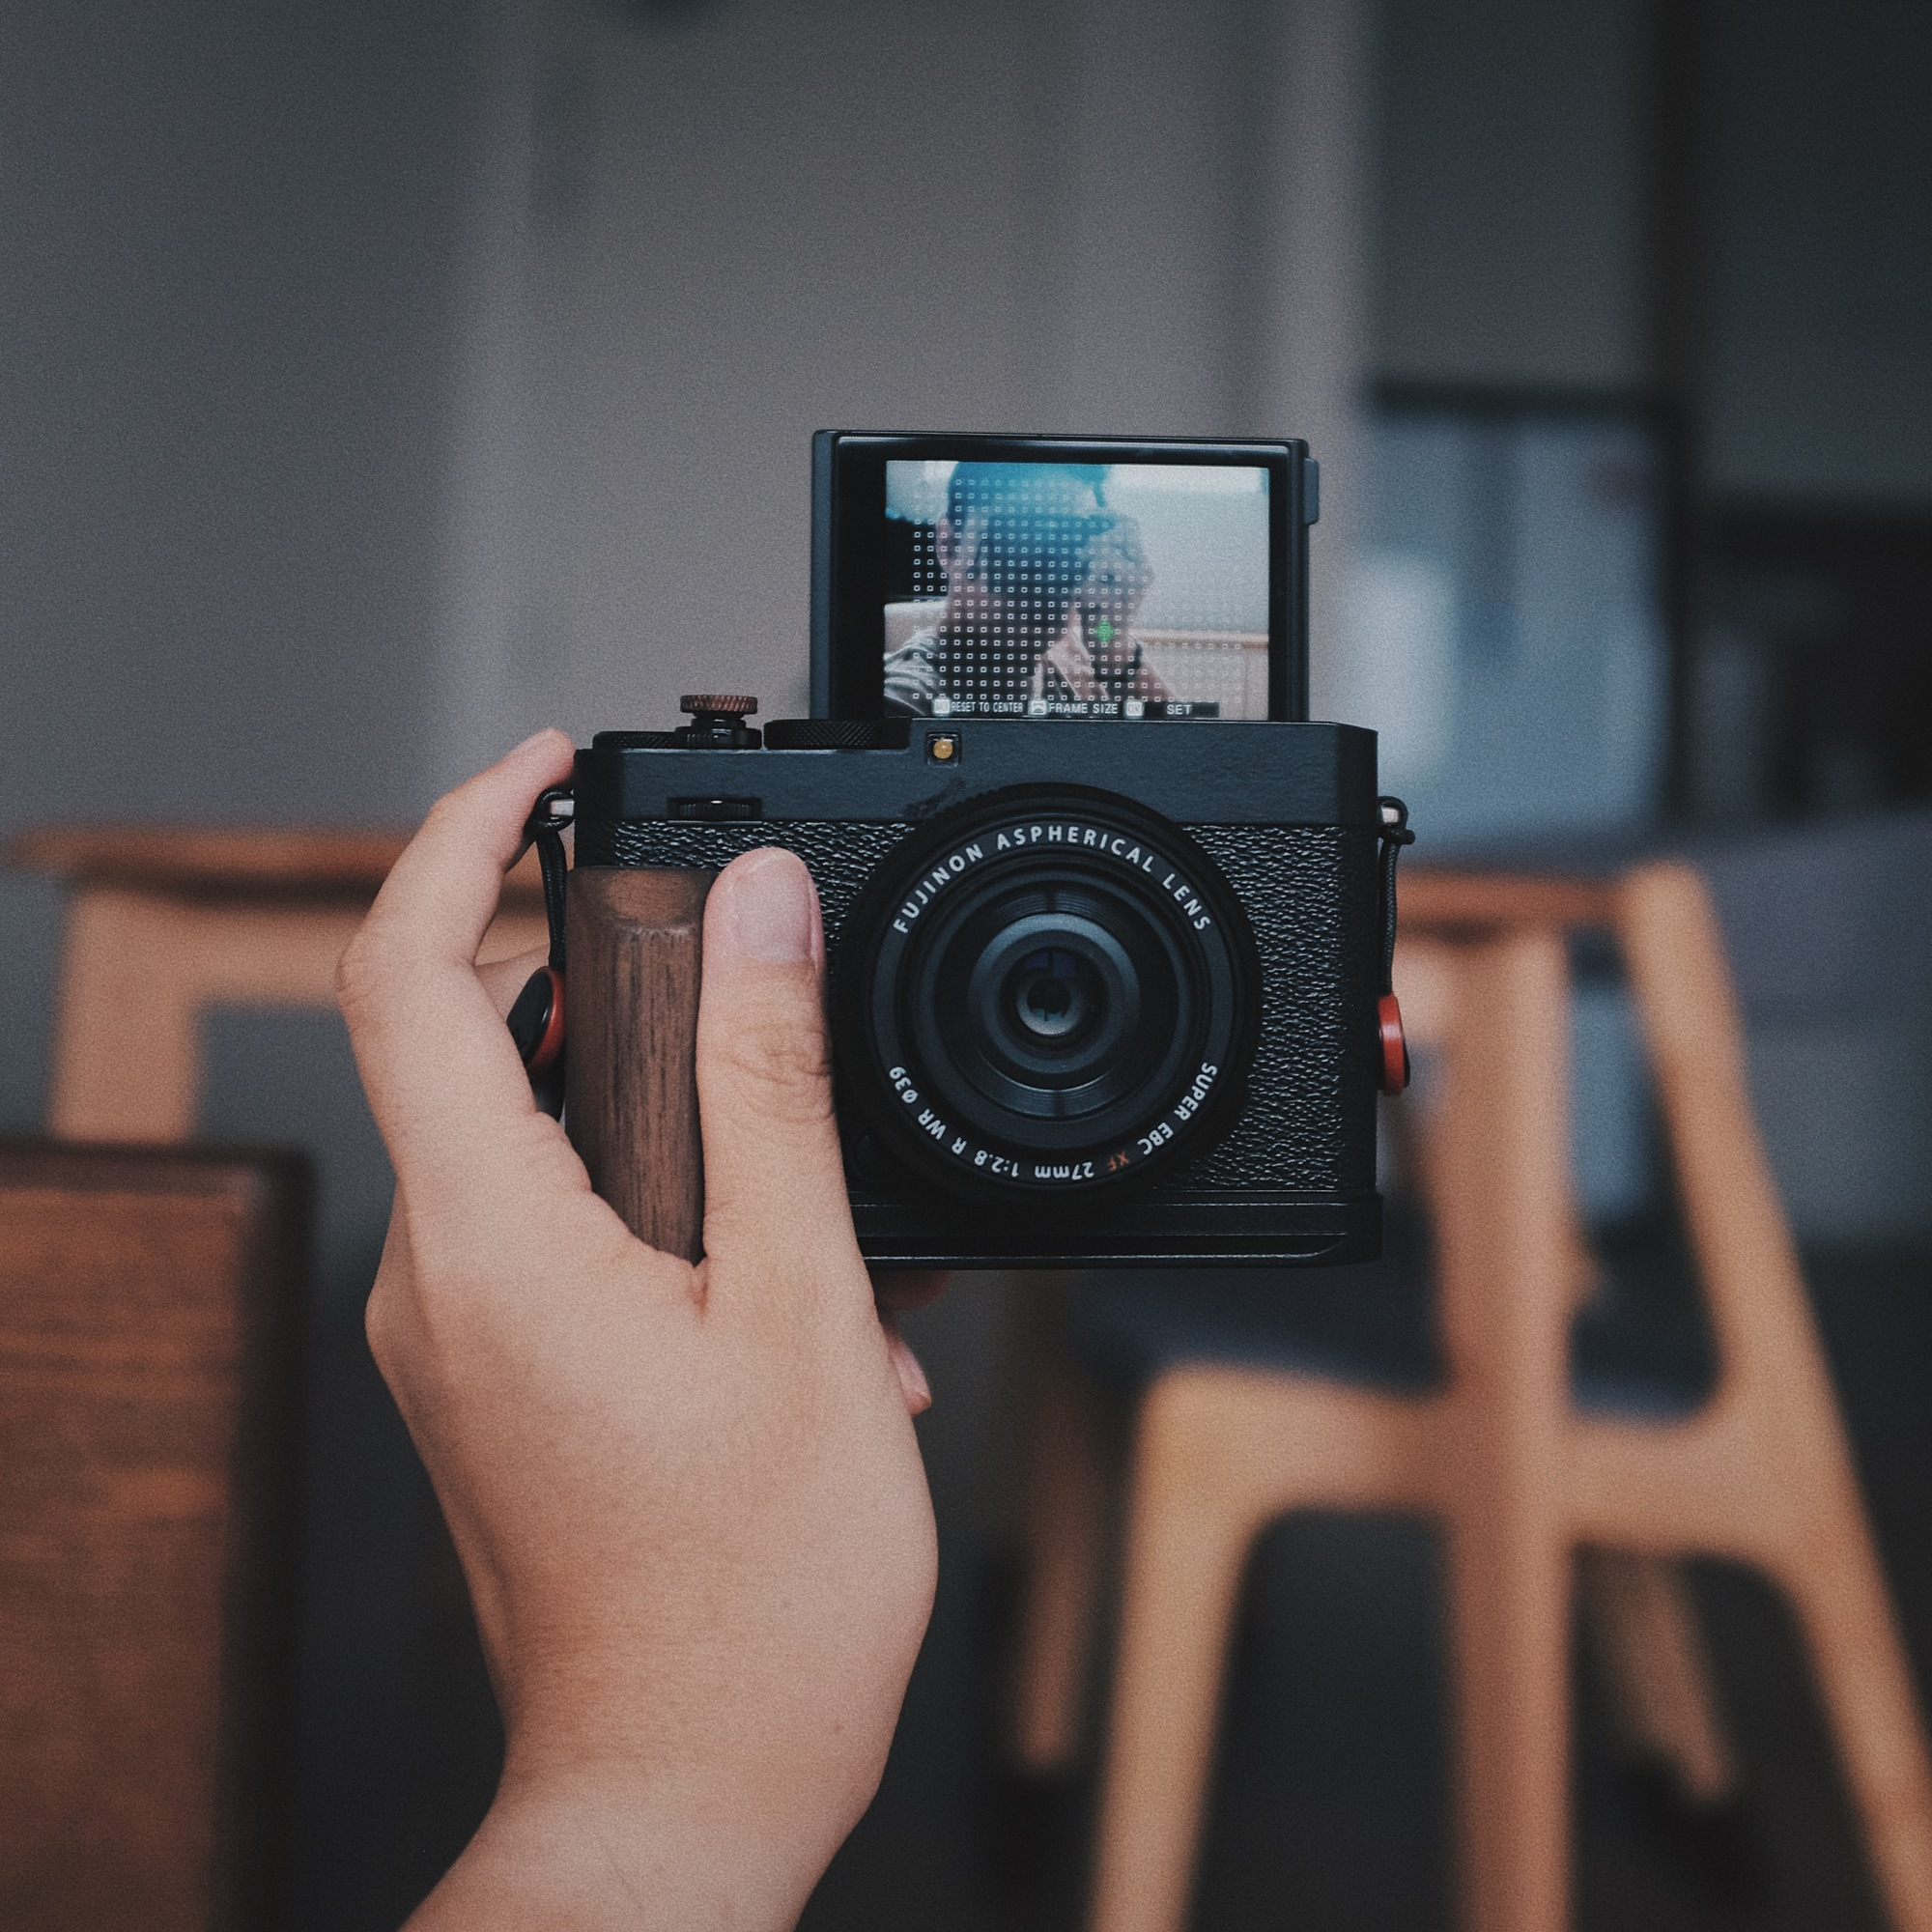
\includegraphics[width=\linewidth]{\envfinaldir/coverpic-prod.jpg}\par
            % \vskip 30pt
            \vfill

            \normalsize\rmfamily\scshape
            \copyright{} The Web Digest Project \hfill\large \envdatestr
        \end{center}
    \end{titlepage}
    % \restoregeometry
}
\newcommand{\simplehref}[1]{%
    \textcolor{blue!80!green}{\href{#1}{#1}}%
}
\renewcommand{\contentsname}{\center\Huge\sffamily\bfseries Contents\par\vskip 20pt}
\newcounter{ipartcounter}
\setcounter{ipartcounter}{0}
\newcommand{\ipart}[1]{
    % \vskip 20pt
    \clearpage
    \stepcounter{ipartcounter}
    \phantomsection
    \addcontentsline{toc}{chapter}{#1}
    % \begin{center}
    %     \Huge
    %     \sffamily\bfseries
    %     #1
    % \end{center}
    % \vskip 20pt plus 7pt
}
\newcounter{ichaptercounter}
\setcounter{ichaptercounter}{0}
\newcommand{\ichapter}[1]{
    % \vskip 20pt
    \clearpage
    \stepcounter{ichaptercounter}
    \phantomsection
    \addcontentsline{toc}{section}{\numberline{\arabic{ichaptercounter}}#1}
    \begin{center}
        \Huge
        \sffamily\bfseries
        #1
    \end{center}
    \vskip 20pt plus 7pt
}
\newcommand{\entrytitlefont}[1]{\subsection*{\raggedright\Large\sffamily\bfseries#1}}
\newcommand{\entryitemGeneric}[2]{
    % argv: title, url
    \parbox{\linewidth}{
        \entrytitlefont{#1}\par\vskip 5pt
        \footnotesize\ttfamily\mdseries
        \simplehref{#2}
    }\vskip 11pt plus 11pt minus 1pt
}
\newcommand{\entryitemGithub}[3]{
    % argv: title, url, desc
    \parbox{\linewidth}{
        \entrytitlefont{#1}\par\vskip 5pt
        \footnotesize\ttfamily\mdseries
        \simplehref{#2}\par\vskip 5pt
        \small\rmfamily\mdseries#3
    }\vskip 11pt plus 11pt minus 1pt
}
\newcommand{\entryitemAp}[3]{
    % argv: title, url, desc
    \parbox{\linewidth}{
        \entrytitlefont{#1}\par\vskip 5pt
        \footnotesize\ttfamily\mdseries
        \simplehref{#2}\par\vskip 5pt
        \small\rmfamily\mdseries#3
    }\vskip 11pt plus 11pt minus 1pt
}
\newcommand{\entryitemHackernews}[3]{
    % argv: title, hnurl, rawurl
    % \parbox{\linewidth}{
    %     \entrytitlefont{#1}\par\vskip 5pt
    %     \footnotesize\ttfamily\mdseries
    %     \simplehref{#3}\par
    %     \textcolor{black!50}{\href{#2}{#2}}
    % }\vskip 11pt plus 11pt minus 1pt
    \begin{minipage}{\linewidth}
            \entrytitlefont{#1}\par\vskip 5pt
            \footnotesize\ttfamily\mdseries
            \simplehref{#3}\par
            \textcolor{black!50}{\href{#2}{#2}}
    \end{minipage}\par\vskip 11pt plus 11pt minus 1pt
}







\begin{document}

\makeheader

\tableofcontents\clearpage




\ipart{Developers}
\ichapter{Hacker News}
\entryitemTwoLinks{How to make the Framework Desktop run even quieter}{https://news.ycombinator.com/item?id=45266039}{https://noctua.at/en/how-to-make-the-framework-desktop-run-even-quieter}

\entryitemTwoLinks{Adios Chicos, 25 Years of KDE}{https://news.ycombinator.com/item?id=45265881}{https://jriddell.org/2025/09/14/adios-chicos-25-years-of-kde/}

\entryitemTwoLinks{Denmark close to wiping out cancer-causing HPV strains after vaccine roll-out}{https://news.ycombinator.com/item?id=45265745}{https://www.gavi.org/vaccineswork/denmark-close-wiping-out-leading-cancer-causing-hpv-strains-after-vaccine-roll-out}

\entryitemTwoLinks{DOJ Deletes Study Showing Domestic Terrorists Are Most Often Right Wing}{https://news.ycombinator.com/item?id=45265462}{https://www.404media.co/doj-deletes-study-showing-domestic-terrorists-are-most-often-right-wing/}

\entryitemTwoLinks{Scammed out of \$130K via fake Google call, spoofed Google email and auth sync}{https://news.ycombinator.com/item?id=45264726}{https://bewildered.substack.com/p/i-was-scammed-out-of-130000-and-google}

\entryitemTwoLinks{Waymo has received our pilot permit allowing for commercial operations at SFO}{https://news.ycombinator.com/item?id=45264562}{https://waymo.com/blog/\#short-all-systems-go-at-sfo-waymo-has-received-our-pilot-permit}

\entryitemTwoLinks{Bertrand Russell to Oswald Mosley (1962)}{https://news.ycombinator.com/item?id=45264340}{https://lettersofnote.com/2016/02/02/every-ounce-of-my-energy/}

\entryitemTwoLinks{Plugin System}{https://news.ycombinator.com/item?id=45264190}{https://iina.io/plugins/}

\entryitemTwoLinks{A new experimental Google app for Windows}{https://news.ycombinator.com/item?id=45263317}{https://blog.google/products/search/google-app-windows-labs/}

\entryitemTwoLinks{The old SF tech scene is dead. What it's morphing into is more sinister}{https://news.ycombinator.com/item?id=45263230}{https://www.sfgate.com/tech/article/bay-area-tech-scene-dorky-now-terrifying-21042943.php}

\entryitemTwoLinks{Microsoft Favors Anthropic over OpenAI for Visual Studio Code}{https://news.ycombinator.com/item?id=45263063}{https://www.theverge.com/report/778641/microsoft-visual-studio-code-anthropic-claude-4}

\entryitemTwoLinks{Things you can do with a Software Defined Radio (2024)}{https://news.ycombinator.com/item?id=45262835}{https://blinry.org/50-things-with-sdr/}

\entryitemTwoLinks{Europe is locking itself in to US LNG}{https://news.ycombinator.com/item?id=45262346}{https://davekeating.substack.com/p/after-escaping-russian-energy-dependence}

\entryitemTwoLinks{Java 25 officially released}{https://news.ycombinator.com/item?id=45261946}{https://mail.openjdk.org/pipermail/announce/2025-September/000360.html}

\entryitemTwoLinks{Generative AI as Seniority-Biased Technological Change}{https://news.ycombinator.com/item?id=45261930}{https://papers.ssrn.com/sol3/papers.cfm?abstract\_id=5425555}

\entryitemTwoLinks{Trucker built a scale model of NYC over 21 years}{https://news.ycombinator.com/item?id=45261877}{https://gothamist.com/arts-entertainment/this-trucker-built-a-scale-model-of-nyc-over-21-years-its-drawing-museums-attention}

\entryitemTwoLinks{When the job search becomes impossible}{https://news.ycombinator.com/item?id=45261848}{https://www.jeffwofford.com/wp/?p=2240}

\entryitemTwoLinks{CIA Freedom of Information Act Electronic Reading Room}{https://news.ycombinator.com/item?id=45261764}{https://www.cia.gov/readingroom}

\entryitemTwoLinks{Just Use HTML}{https://news.ycombinator.com/item?id=45261480}{https://gomakethings.com/just-use-html/}

\entryitemTwoLinks{Man jailed for parole violations after refusing to decrypt his Tor node}{https://news.ycombinator.com/item?id=45261163}{https://reddit.com/r/TOR/comments/1ni5drm/the\_fbi\_couldnt\_get\_my\_husband\_to\_decrypt\_his\_tor/}\ichapter{Phoronix}
\entryitemGeneric{\hskip 0pt{}Tyr Driver Being Submitted For Linux 6.18 As Rust-Based Arm Mali Driver}{https://www.phoronix.com/news/Rust-DRM-Drivers-Linux-6.18-Tyr}

\entryitemGeneric{\hskip 0pt{}AMD Begins Plumbing APCI C4 Support In The Linux Kernel For Greater Power Savings}{https://www.phoronix.com/news/AMD-ACPI-C4-Linux-Kernel-Code}

\entryitemGeneric{\hskip 0pt{}Intel Xeon 6980P "Granite Rapids" Linux Performance One Year Later}{https://www.phoronix.com/review/intel-xeon-6980p-2025}

\entryitemGeneric{\hskip 0pt{}AMD ROCm 7.0 Officially Released With Many Significant Improvements}{https://www.phoronix.com/news/AMD-ROCm-7.0-Released}

\entryitemGeneric{\hskip 0pt{}Fedora 43 Beta ISOs Released For Testing This Leading-Edge Linux OS}{https://www.phoronix.com/news/Fedora-43-Beta-Released}

\entryitemGeneric{\hskip 0pt{}AMD ROCm 7.0 Begins Rocking Out On GitHub}{https://www.phoronix.com/news/AMD-ROCm-7.0-Rolling-Out}

\entryitemGeneric{\hskip 0pt{}Fedora Workstation 43 Beta Is Running Well On AMD Strix Halo / Framework Desktop}{https://www.phoronix.com/review/fedora-43-beta}

\entryitemGeneric{\hskip 0pt{}Intel USBIO USB IO Expander Drivers Expected To Be Merged For Linux 6.18}{https://www.phoronix.com/news/Intel-USBIO-USB-Drivers-6.18}

\entryitemGeneric{\hskip 0pt{}Linux Patches Posted For Enabling The Tenstorrent Blackhole SoC}{https://www.phoronix.com/news/Linux-Blackhole-SoC-Patches}


\ipart{Developers~~~~(zh-Hans)}
\ichapter{Solidot}
\entryitemGeneric{\hskip 0pt{}蚁后被发现产下了两个不同物种的蚂蚁}{https://www.solidot.org/story?sid=82326}

\entryitemGeneric{\hskip 0pt{}AOMedia 联盟将于年底发布 AV2 编解码器}{https://www.solidot.org/story?sid=82325}

\entryitemGeneric{\hskip 0pt{}Godot 4.5 释出}{https://www.solidot.org/story?sid=82324}

\entryitemGeneric{\hskip 0pt{}Microsoft 365 应用将从下个月起强制安装 Copilot Chat}{https://www.solidot.org/story?sid=82323}

\entryitemGeneric{\hskip 0pt{}Google 改变了 Android 的安全更新模式}{https://www.solidot.org/story?sid=82322}

\entryitemGeneric{\hskip 0pt{}中美达成交易 TikTok 美国业务的初步框架协议}{https://www.solidot.org/story?sid=82321}

\entryitemGeneric{\hskip 0pt{}非洲岛民向政府投诉结果被罚断网一年}{https://www.solidot.org/story?sid=82320}

\entryitemGeneric{\hskip 0pt{}印度 IT 外包行业大幅减少招聘应届生}{https://www.solidot.org/story?sid=82319}

\entryitemGeneric{\hskip 0pt{}英伟达被指违反中国反垄断法}{https://www.solidot.org/story?sid=82318}

\entryitemGeneric{\hskip 0pt{}步行量而不是强度与更低的慢性背痛风险相关}{https://www.solidot.org/story?sid=82317}

\entryitemGeneric{\hskip 0pt{}LIGO 成为黑洞狩猎机器}{https://www.solidot.org/story?sid=82316}

\entryitemGeneric{\hskip 0pt{}韩国扫地机器人试图通过差异化与中国公司竞争}{https://www.solidot.org/story?sid=82315}

\entryitemGeneric{\hskip 0pt{}全球人口正以更快的速度收缩}{https://www.solidot.org/story?sid=82314}

\entryitemGeneric{\hskip 0pt{}日本老年人口比例占到 29.4\%}{https://www.solidot.org/story?sid=82313}

\entryitemGeneric{\hskip 0pt{}CRISPR 基因编辑的马引发争议}{https://www.solidot.org/story?sid=82312}

\entryitemGeneric{\hskip 0pt{}日本百岁人口数量接近 10 万}{https://www.solidot.org/story?sid=82311}

\entryitemGeneric{\hskip 0pt{}NewsGuard 的调查显示 AI 生成虚假信息的比例一年内翻了一倍}{https://www.solidot.org/story?sid=82310}

\entryitemGeneric{\hskip 0pt{}AMD 的 RDNA4 GPU 架构}{https://www.solidot.org/story?sid=82309}

\entryitemGeneric{\hskip 0pt{}2025 年度拉斯克医学奖揭晓}{https://www.solidot.org/story?sid=82308}

\entryitemGeneric{\hskip 0pt{}阿联酋发布能与 DeepSeek 竞争的开源模型}{https://www.solidot.org/story?sid=82307}\ichapter{V2EX}
\entryitemGeneric{\hskip 0pt{}[程序员] 切回 Chrome 时偶尔界面卡顿}{https://www.v2ex.com/t/1159790}

\entryitemGeneric{\hskip 0pt{}[Rust] 介绍一个 like rails 的 rust 框架。 性能和开发速度都快。}{https://www.v2ex.com/t/1159789}

\entryitemGeneric{\hskip 0pt{}[摄影] 西部雪鸻}{https://www.v2ex.com/t/1159788}

\entryitemGeneric{\hskip 0pt{}[iOS] ios26 太棒了}{https://www.v2ex.com/t/1159787}

\entryitemGeneric{\hskip 0pt{}[Solana] 20250916 - 优化了打赏流程的速度}{https://www.v2ex.com/t/1159786}

\entryitemGeneric{\hskip 0pt{}[分享发现] @z.org 邮箱,超短 2 字符别名开注}{https://www.v2ex.com/t/1159785}

\entryitemGeneric{\hskip 0pt{}[分享创造] 诚邀,上线了一个树洞或者社交应用(?)}{https://www.v2ex.com/t/1159784}

\entryitemGeneric{\hskip 0pt{}[VPS] 搬瓦工 THE-PLAN-V1 连我的手机(S24+)的加解密都不如}{https://www.v2ex.com/t/1159783}

\entryitemGeneric{\hskip 0pt{}[Apple] 更新 iOS26 之后,大家的「有线配件」连接选项还能修改吗}{https://www.v2ex.com/t/1159782}

\entryitemGeneric{\hskip 0pt{}[Go 编程语言] go build 时如何才能不携带 BuildInfo 信息?}{https://www.v2ex.com/t/1159780}

\entryitemGeneric{\hskip 0pt{}[分享创造] 写了个简单的网站转 RSS 的 worker}{https://www.v2ex.com/t/1159779}

\entryitemGeneric{\hskip 0pt{}[服务器] 求推荐海外独立服务器}{https://www.v2ex.com/t/1159778}

\entryitemGeneric{\hskip 0pt{}[创业组队] 🎾 体育 AI 公司 寻找一名安卓专家}{https://www.v2ex.com/t/1159777}

\entryitemGeneric{\hskip 0pt{}[问与答] 我的 xbox one 手柄到底是国产的么?}{https://www.v2ex.com/t/1159776}

\entryitemGeneric{\hskip 0pt{}[职场话题] 感觉自己是不是有什么精神洁癖}{https://www.v2ex.com/t/1159775}

\entryitemGeneric{\hskip 0pt{}[macOS] macOS 26 无法修改 mac 地址}{https://www.v2ex.com/t/1159773}

\entryitemGeneric{\hskip 0pt{}[职场话题] 果然世界就是一个巨大的草台班子,大公司也避免不了}{https://www.v2ex.com/t/1159771}

\entryitemGeneric{\hskip 0pt{}[南京] 南京玄武区的酒店,国庆节紧张吗?}{https://www.v2ex.com/t/1159770}

\entryitemGeneric{\hskip 0pt{}[分享创造] 你的 MCP 服务器正在被重复启动 5 次 - 这里有个解决方案}{https://www.v2ex.com/t/1159769}

\entryitemGeneric{\hskip 0pt{}[分享创造] 我做了个大模型 API 聚合网关 evolink.ai,帮你解决 API 不稳定和价格波动两大难题}{https://www.v2ex.com/t/1159768}

\entryitemGeneric{\hskip 0pt{}[Safari] macOS 15.7, Safari 升级到最新版后,紧凑模式下标签页的地址栏不能编辑了,有遇到的吗?}{https://www.v2ex.com/t/1159767}

\entryitemGeneric{\hskip 0pt{}[宽带症候群] 家里路由器时不时断网,请教如何排查}{https://www.v2ex.com/t/1159766}

\entryitemGeneric{\hskip 0pt{}[iPadOS] iPad OS 26 的多任务管理有点意思}{https://www.v2ex.com/t/1159765}

\entryitemGeneric{\hskip 0pt{}[Apple] iOS26 海外评价真的好,自动翻译}{https://www.v2ex.com/t/1159763}

\entryitemGeneric{\hskip 0pt{}[Android] 如何修改微信实时定位?}{https://www.v2ex.com/t/1159762}

\entryitemGeneric{\hskip 0pt{}[OpenAI] 购买了 plus 后,感觉回答反而变慢了很多}{https://www.v2ex.com/t/1159761}

\entryitemGeneric{\hskip 0pt{}[iPhone] 有人给 iPhone14 pro 升级到 iOS 26 吗?}{https://www.v2ex.com/t/1159759}

\entryitemGeneric{\hskip 0pt{}[程序员] 感觉现在接触的 AI 知识很是细碎,大家手里有没有系统性的知识学习方法?}{https://www.v2ex.com/t/1159758}

\entryitemGeneric{\hskip 0pt{}[程序员] 垃圾电信把我的 udp 包全丢了}{https://www.v2ex.com/t/1159757}

\entryitemGeneric{\hskip 0pt{}[iOS] [投票]升级 IOS 26 的扣 1,不打算升的扣 0,观望的扣 2}{https://www.v2ex.com/t/1159756}

\entryitemGeneric{\hskip 0pt{}[分享发现] 被宽带限速的可以进来测试下方法}{https://www.v2ex.com/t/1159755}

\entryitemGeneric{\hskip 0pt{}[NAS] 继续学习:关于文件存储}{https://www.v2ex.com/t/1159754}

\entryitemGeneric{\hskip 0pt{}[分享创造] 用一个知识点构建一个虚拟世界}{https://www.v2ex.com/t/1159753}

\entryitemGeneric{\hskip 0pt{}[问与答] 小城市一次性交 9 万,每个月领 1200,以后可以一直领,这个靠谱吗?}{https://www.v2ex.com/t/1159752}

\entryitemGeneric{\hskip 0pt{}[旅行] 全世界最搞笑的一周!日本综艺节目「大阪喜剧节 2025」于 9/15(一)~ 9/21(日)举行!大阪旅游亮点不容错过!}{https://www.v2ex.com/t/1159751}

\entryitemGeneric{\hskip 0pt{}[宽带症候群] 上海电信精品网拨不到 58.32 段了?}{https://www.v2ex.com/t/1159750}

\entryitemGeneric{\hskip 0pt{}[Cursor] cursor 的 claude-4-sonnet 是不是挂了}{https://www.v2ex.com/t/1159749}

\entryitemGeneric{\hskip 0pt{}[macOS] macos 双微信,升级系统不好用。 wechat-2.sh 解决}{https://www.v2ex.com/t/1159748}

\entryitemGeneric{\hskip 0pt{}[macOS] macOS 26,用什么菜单栏管理软件?}{https://www.v2ex.com/t/1159746}

\entryitemGeneric{\hskip 0pt{}[酷工作] 杭州 Java 研发还有几个 HC}{https://www.v2ex.com/t/1159745}

\entryitemGeneric{\hskip 0pt{}[生活] 是我太过不相信他人了吗?}{https://www.v2ex.com/t/1159744}

\entryitemGeneric{\hskip 0pt{}[分享创造] Vibe 了一个 Spelling Bee 游戏的自动答案网站和插件}{https://www.v2ex.com/t/1159743}

\entryitemGeneric{\hskip 0pt{}[macOS] Mac 续航测试}{https://www.v2ex.com/t/1159742}

\entryitemGeneric{\hskip 0pt{}[问与答] 怎么查一个城市民航客机的航线图?}{https://www.v2ex.com/t/1159741}

\entryitemGeneric{\hskip 0pt{}[Apple] 有购买了新的 40w 充电头的 macbook pro 用户吗?}{https://www.v2ex.com/t/1159740}

\entryitemGeneric{\hskip 0pt{}[分享发现] 👉🏻 CognitiveKernel-Launchpad: 5 分钟,我搭出了自己的第一个 AI Agent 👈🏻}{https://www.v2ex.com/t/1159739}

\entryitemGeneric{\hskip 0pt{}[加密货币] 今天搞了一个 okx 的自动化交易机器人, 主要是用 AI 做决策+调 okx 接口执行合约交易, 目前胜率很感人, 稳定在-100\%, 给大家解解闷.}{https://www.v2ex.com/t/1159737}

\entryitemGeneric{\hskip 0pt{}[Apple] macOS 26 chrome 全屏后右键标签页没反应}{https://www.v2ex.com/t/1159736}

\entryitemGeneric{\hskip 0pt{}[分享发现] Claude Code 免费白嫖 2 天,不用白不用}{https://www.v2ex.com/t/1159735}

\entryitemGeneric{\hskip 0pt{}[问与答] 如何确定自己是否需要港版 iPhone}{https://www.v2ex.com/t/1159734}


\ipart{Generic News}







\clearpage
\leavevmode\vfill
\footnotesize

Copyright \copyright{} 2023-2025 Neruthes and other contributors.

This document is published with CC BY-NC-ND 4.0 license.

The entries listed in this newsletter may be copyrighted by their respective creators.

This newsletter is generated by the Web Digest project.

The newsletters are also delivered via Telegram channel \CJKunderline{\href{https://t.me/webdigestchannel}{https://t.me/webdigestchannel}}.\\
RSS feed is available at \CJKunderline{\href{https://webdigest.pages.dev/rss.xml}{https://webdigest.pages.dev/rss.xml}}.

This newsletter is available in PDF at
\CJKunderline{\href{https://webdigest.pages.dev/}{https://webdigest.pages.dev/}}.

The source code being used to generate this newsletter is available at\\
\CJKunderline{\href{https://github.com/neruthes/webdigest}{https://github.com/neruthes/webdigest}}.

This newsletter is also available in
\CJKunderline{\href{http://webdigest.pages.dev/readhtml/\envyear/WebDigest-20250917.html}{HTML}} and
\CJKunderline{\href{https://github.com/neruthes/webdigest/blob/master/markdown/\envyear/WebDigest-20250917.md}{Markdown}}.


\coverpic{https://unsplash.com/photos/vCsK47Vi0CM}{Steve Johnson}


\end{document}
